\section{Introduction}

\subsection{Shughni}
The Shughni language (ISO: sgh; Glottolog: shug1248) is a language of the Iranian branch of the Indo-European family \parencite[12]{plungian_study_2022}. As of June 1997, it was estimated to be spoken by approximately 100,000 people \parencite[225]{edelman_languages_1999} in the territories of Tajikistan and Afghanistan. Both countries have a subregion where Shughni is the most widely spoken native language. The Shughni-speaking subregion of Tajikistan is called `Shughnon' and it belongs the to `Gorno-Badakhshan Autonomus' province. In Afghanistan, the Shughni-speaking region is called `Shughnan' and it lies within the territory of `Badakhshan' province \parencite[2]{parker_shughni_2023}. Shughni belongs to `Pamiri' areal language group, which is spoken along the Panj river in Pamir Mountains area.
\begin{figure}[h]
    \centering
    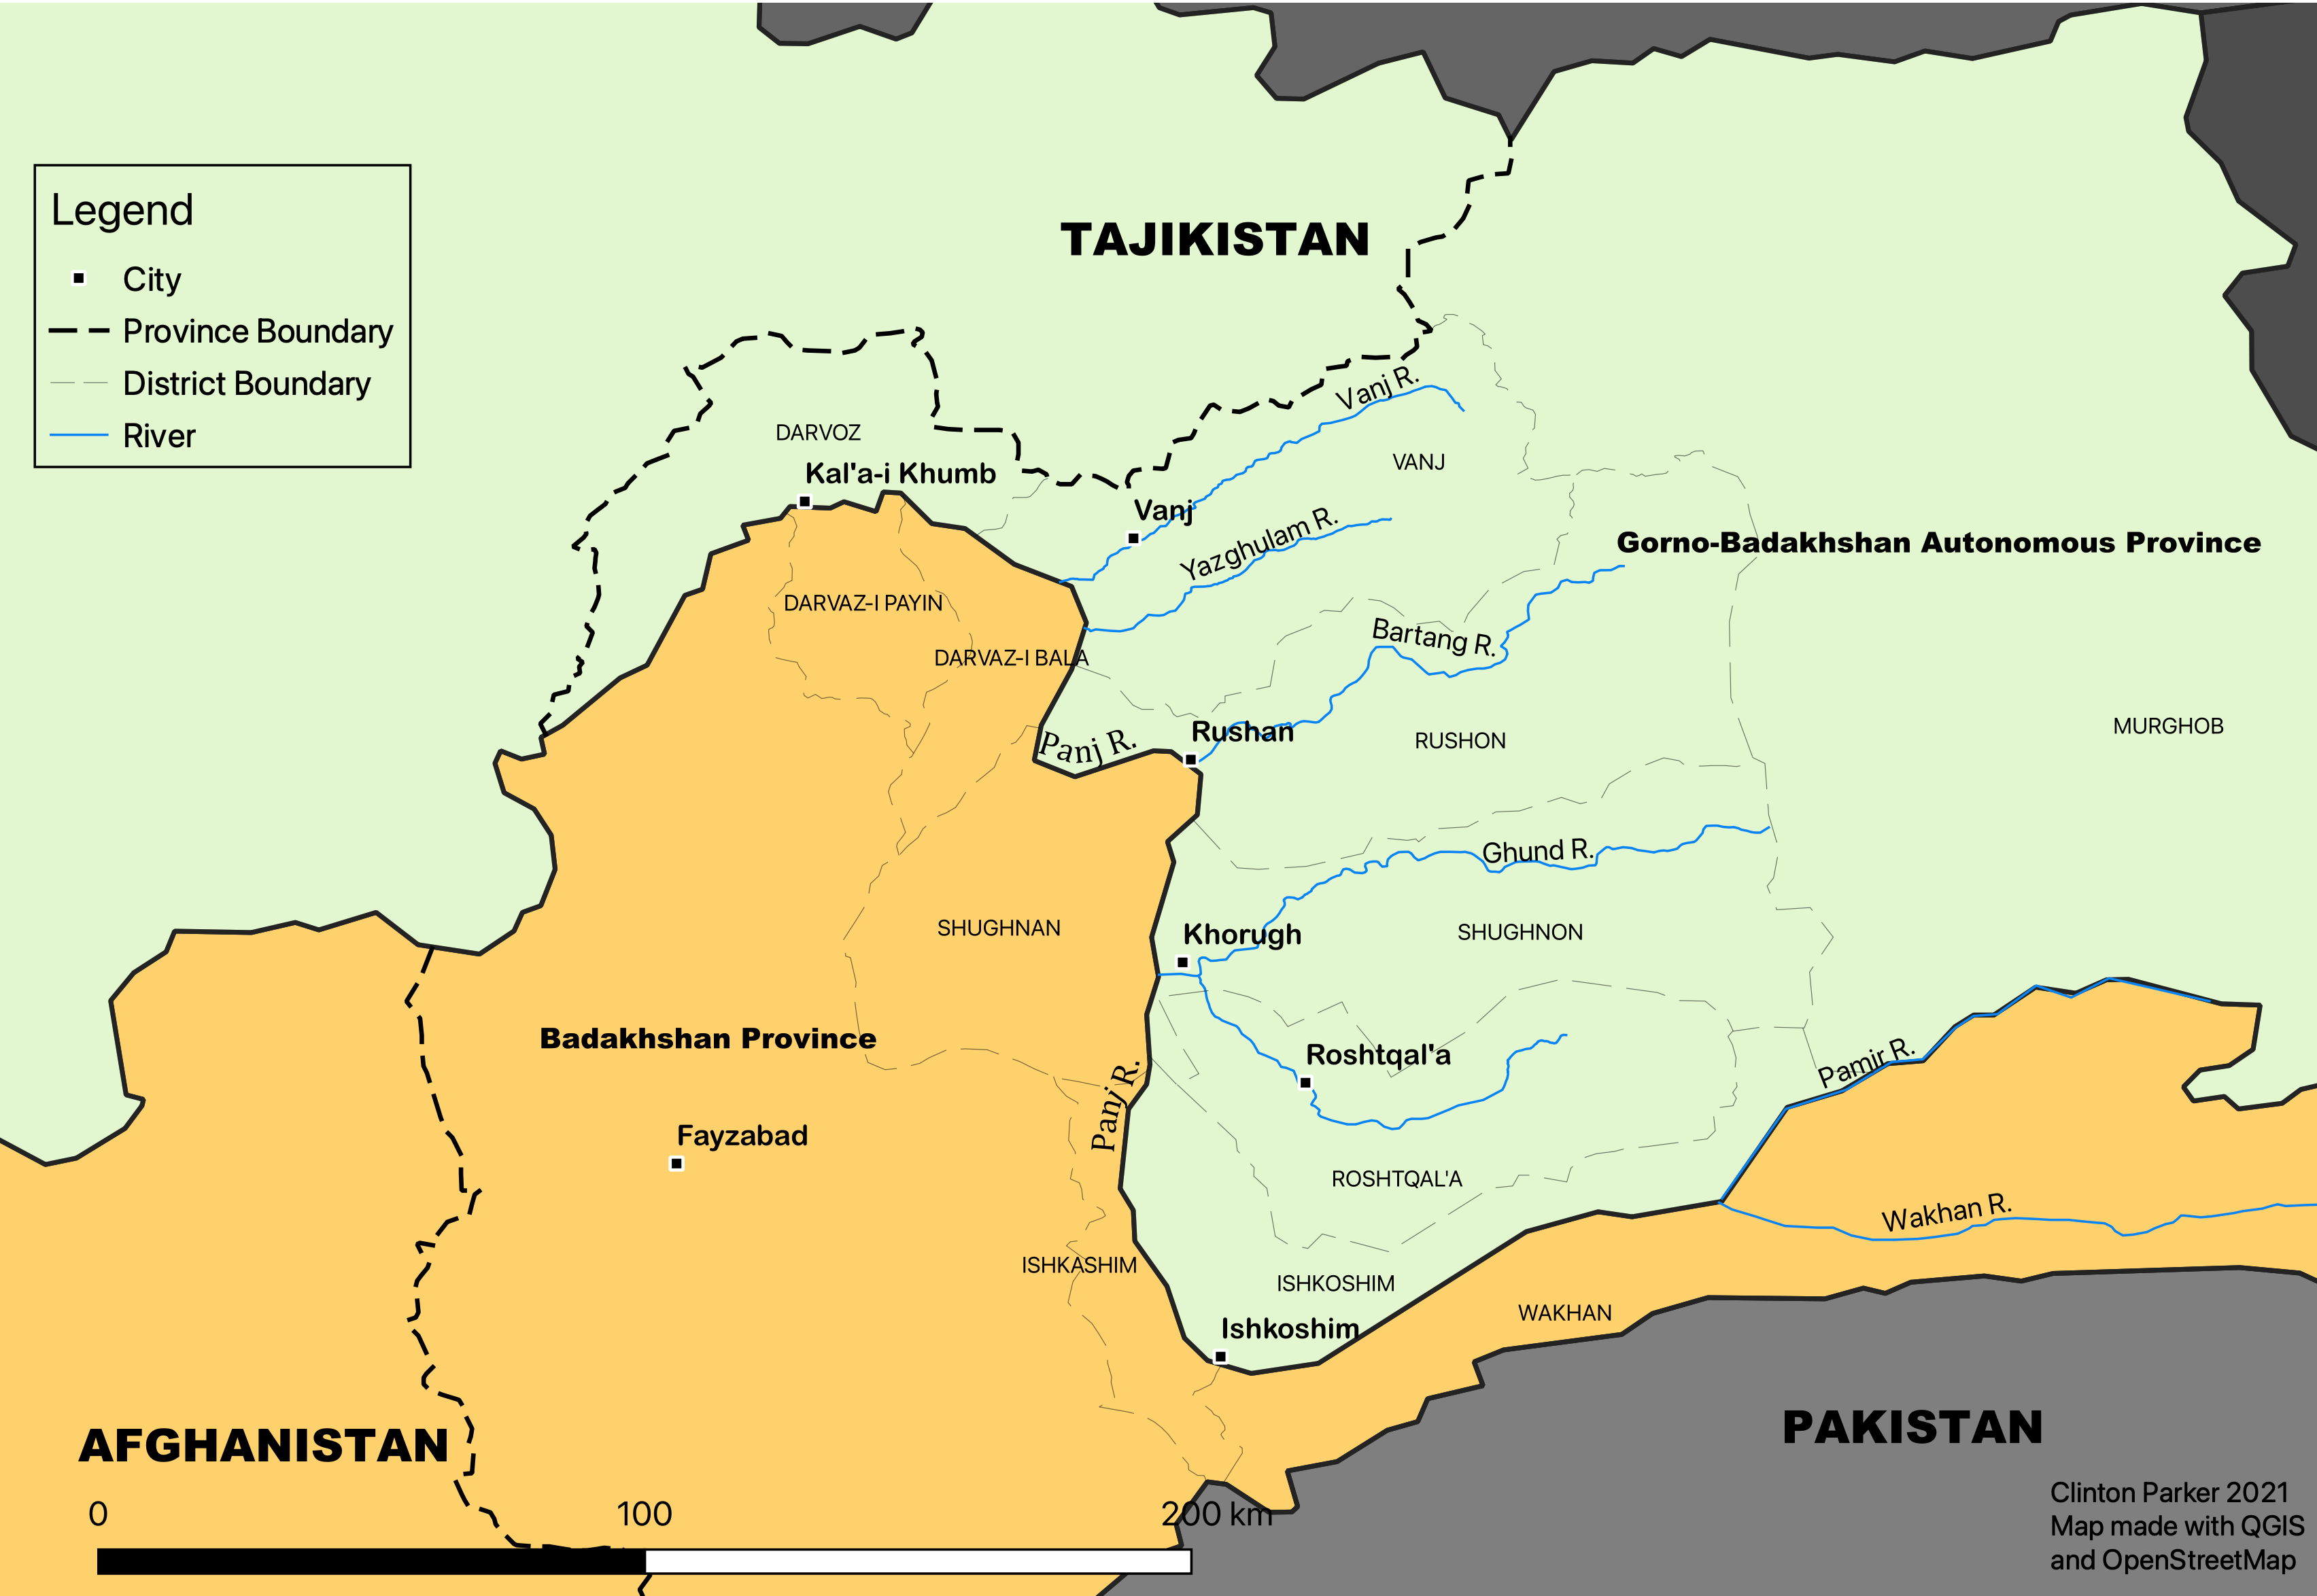
\includegraphics[scale=0.125]{\rootdir/img/map.png}
    \caption{Mountainous Badakhshan Autonomous Province of Tajikistan and Badakhshan Province of Afghanistan, \parencite[Fig 1.1]{parker_shughni_2023}}
    \label{fig:map1}
\end{figure}

There are three alphabets for Shughni that were derived from Cyrillic, Arabic and Latin scripts. Geographically the usage of said scripts correspond to the dominant script of each country where Shughni is spoken. In Tajikistan both official languages (Tajik and Russian) use Cyrillic script, so does Shughni on territory of Tajikistan. In Afghanistan Arabic script is used in Shughni, matching official languages (Pashto and Dari). 

Latin script was developed and used in Tajikistan in 1930s \parencite[226]{edelman_languages_1999} \parencite[788]{edelman_dodykhudoeva_shughni_2009}, but according to \textcite{edelman_languages_1999} was not widely adapted. Later around 1980s a Cyrillic script gained popularity in Tajikistan, having some poetic literature and school materials based on Tajik's alphabet, which is Cyrillic \parencite{edelman_languages_1999}. Today, Latin script is mostly used by researchers in scientific works.

The morphological parser developed in this work is based on materials that focus on Shughni spoken in Tajikistan. All the base lexicon is Cyrillic and comes from dictionaries that cover Shughni in `Gorno-Badakhshan Autonomus Province'. Latin script is supported with the help of transliteration.

\todo{Вы ничего не пишите про диалектное членение, возможно оно есть, например, в Афганистане.}

\subsection{Morphology modeling}
Today there are two general approaches to the task of morphology modeling. The deep learning (DL) approach and the rule-based approach. 

The DL approach today typically makes use of training transformer models like \texttt{BERT} \parencite{devlin_2019} on vast amounts of marked-up data. This task becomes challenging, considering that Shughni is a low-resource language, meaning it lacks digital textual data. Although, DL approach was not utilized in this work, some existing DL approaches for low-resource languages are covered in section \ref{dl_methods}.

With the rule-based approach, morphological model is being built by writing grammar rules using some formalism language and by listing base lexicon. In this work, rule-based approach was utilized, as it does not depend on the amount of available marked-up data as the DL approach does. It requires lexicons and morphological grammar descriptions, which exist for Shughni and which are discussed in Section \ref{data_section}.

\todo{Я бы считал, что корпус тоже нужен, так как только благадаря нему можно хотья как-то направлять разработку, не плутая впотьмах воображения авторов грамматики.}